\documentclass[11pt]{article}
\usepackage[utf8]{inputenc}
\usepackage{graphicx}
\usepackage{geometry}
\usepackage{hyperref}
\usepackage{booktabs}
\usepackage{algorithm}
\usepackage{algpseudocode}
\usepackage{amsmath}
\usepackage{float}
\usepackage{tikz}
\usetikzlibrary{shapes.geometric, arrows.meta, positioning}
\geometry{a4paper, margin=1in}

\title{AgriTech Quality Control System - Assignment 3}
\author{AgriTech CV Team}
\date{\today}

\begin{document}
\maketitle

\begin{abstract}
This report details the implementation of feature-based computer vision methods for the AgriTech SeedCounter project, specifically deploying Canny and Sobel edge detection on two diverse datasets: an agricultural seed dataset originally processed using classical clustering techniques, and the complex BSDS500 natural scene dataset. By replacing the previous clustering methods with edge detection methodologies, we evaluate the generalized performance of these feature extractors. The results indicate that while edge detection (particularly Canny) delivers robust, thin, and continuous closed boundary delineations crucial for high-accuracy object accounting on seeds, these parameters often over-prescribe edges inside highly textured natural images. Overall, the Canny method consistently outperformed the Sobel operator.
\end{abstract}

\section{Introduction \& Background}
In Assignment 2, a robust preprocessing and clustering pipeline was formulated for seed segmentation. While successful, its performance faltered under extreme overlapping and poor lighting conditions where boundaries blur together. Thus, this assignment explores the potential of extracting boundary-specific features—namely, using Canny and Sobel operators—to more precisely delineate objects natively. It also evaluates how well these algorithms generalize from a simple uniform agricultural testbed to a dataset of completely unconstrained natural scenes (BSDS500).

\section{Methodology}
Our dual-dataset processing engine relied heavily upon extracting explicit edge maps from grayscale, Gaussian-blurred inputs (to suppress textural artifacts before calculating gradients). 

\begin{figure}[H]
    \centering
    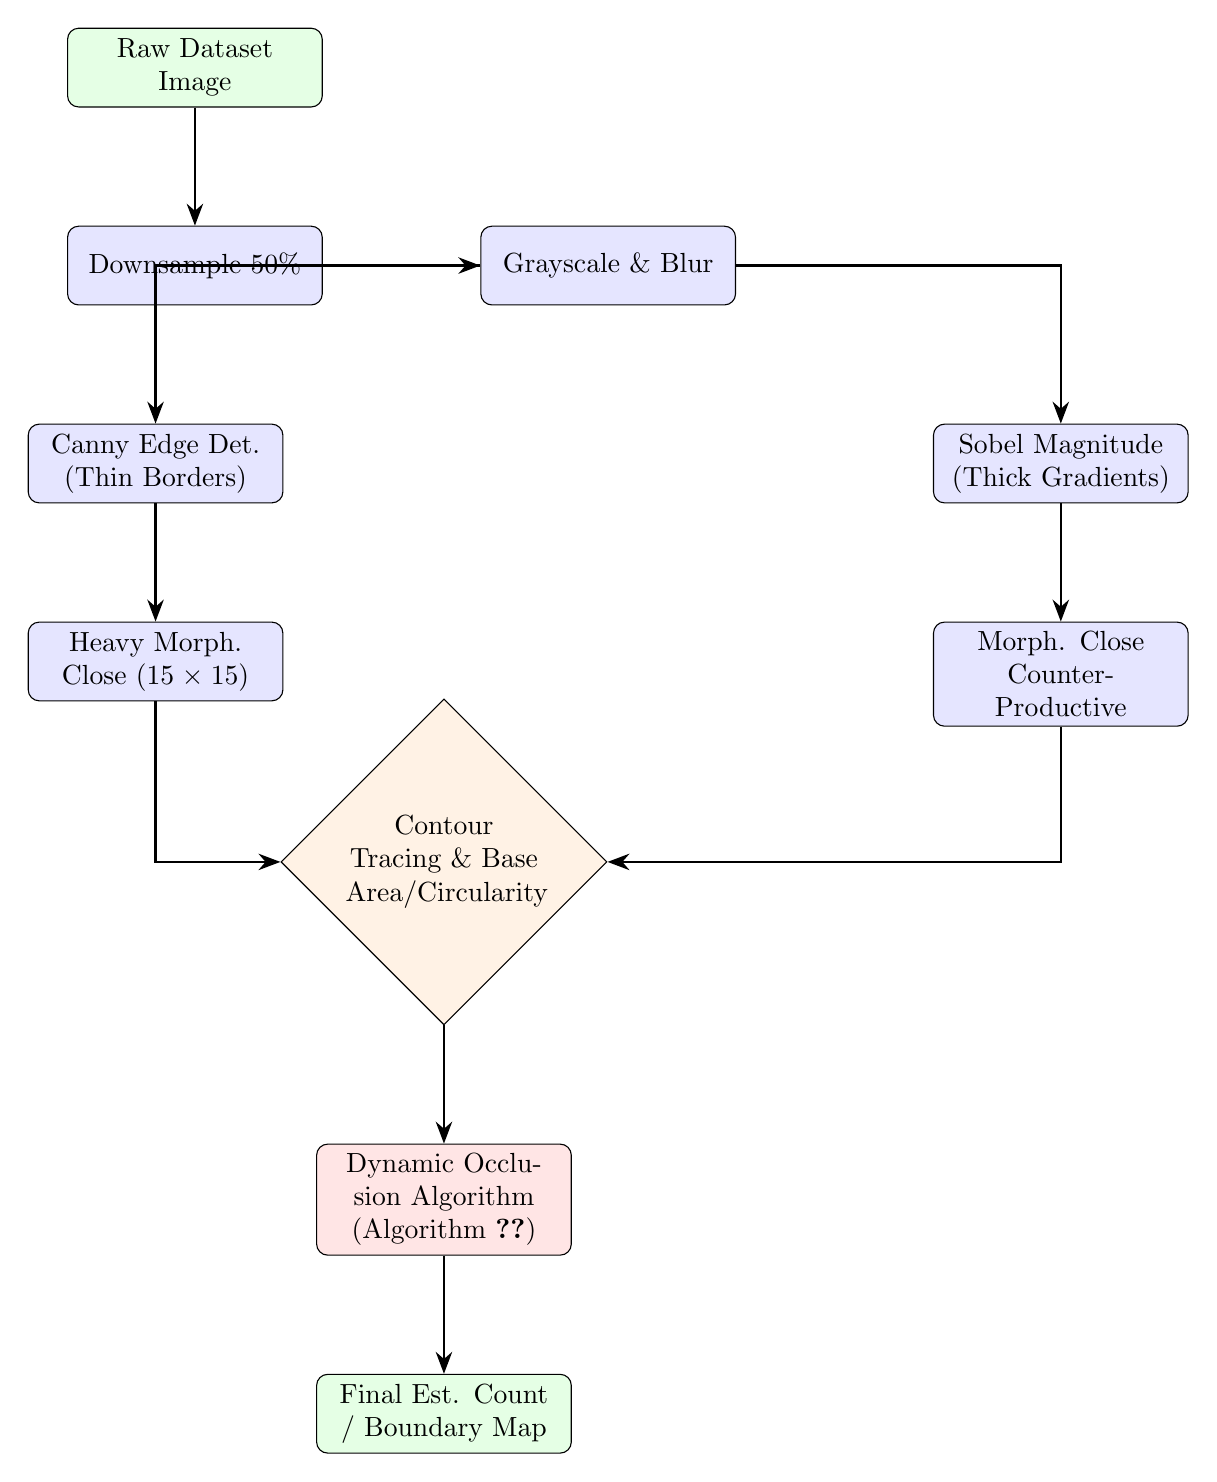
\begin{tikzpicture}[
        node distance=1.5cm and 2cm,
        box/.style={rectangle, draw, rounded corners, text width=3cm, align=center, minimum height=1cm, fill=blue!10},
        decision/.style={diamond, draw, text width=2.5cm, align=center, fill=orange!10},
        arrow/.style={-{Stealth[scale=1.2]}, thick}
    ]
        
    % Nodes
    \node[box, fill=green!10] (input) {Raw Dataset Image};
    \node[box, below=of input] (downsample) {Downsample 50\%};
    \node[box, right=of downsample] (gray) {Grayscale \& Blur};
    
    \node[box, below left=of gray, xshift=-0.5cm] (canny) {Canny Edge Det.\\(Thin Borders)};
    \node[box, below right=of gray, xshift=0.5cm] (sobel) {Sobel Magnitude\\(Thick Gradients)};
    
    \node[box, below=of canny] (morph1) {Heavy Morph. Close ($15\times15$)};
    \node[box, below=of sobel] (morph2) {Morph. Close Counter-Productive};
    
    \node[decision, below right=of morph1, xshift=-1cm, yshift=0.5cm] (contour) {Contour Tracing \& Base Area/Circularity};
    
    \node[box, fill=red!10, below=of contour] (algo) {Dynamic Occlusion Algorithm (Algorithm \ref{alg:occlusion})};
    
    \node[box, fill=green!10, below=of algo] (output) {Final Est. Count / Boundary Map};
    
    % Arrows
    \draw[arrow] (input) -- (downsample);
    \draw[arrow] (downsample) -- (gray);
    \draw[arrow] (gray) -| (canny);
    \draw[arrow] (gray) -| (sobel);
    \draw[arrow] (canny) -- (morph1);
    \draw[arrow] (sobel) -- (morph2);
    \draw[arrow] (morph1) |- (contour);
    \draw[arrow] (morph2) |- (contour);
    \draw[arrow] (contour) -- (algo);
    \draw[arrow] (algo) -- (output);
    
    \end{tikzpicture}
    \caption{Functional logic flow of the feature-based computer vision tracking pipeline.}
    \label{fig:pipeline}
\end{figure}

\subsection{Edge Extraction \& Morphological Bridging}
Initial experiments rapidly demonstrated that standard edge mapping produced disjointed perimeters, causing seeds to fracture into multiple unassociated contours.
\begin{itemize}
    \item \textbf{Canny Edge Detection}: To connect Canny's characteristically thin edges, we deployed dynamically scaled thresholds paired with a heavy $15\times15$ morphological closing operation (dilation followed by erosion). This successfully bridged minute gaps across seed bodies.
    \item \textbf{Sobel Method}: We extracted magnitude gradients utilizing a $3\times3$ kernel. However, owing to Sobel's inherent "thick" gradient nature, standard morphological closing proved counter-productive over highly dense clusters, demanding stricter thresholding to maintain discrete objects.
\end{itemize}

\subsection{Object Counting: Area Estimation \& Circularity Tuning}
The immediate flaw in traditional counting (1 closed contour = 1 seed) manifested during occlusion. When two or more seeds overlapped tightly, edge detectors often traced their collective boundary instead of the intersecting gradients. 

\textbf{Dynamic Occlusion Algorithm:} Through our experiments, we discovered that dividing a massive cluster's total area by a fixed global value grossly underestimated or overestimated counts depending on image-specific scaling. Instead, we implemented a dual-pass dynamic algorithm (documented formally in Algorithm \ref{alg:occlusion}). In the first pass, we calculated the median area exclusively from \textit{highly circular} single isolated seeds to determine the sample's inherent "typical area". In the second pass, any contour possessing an area greater than $1.6\times$ this typical median was mathematically divided by the typical area to yield an estimated localized cluster count. 

\begin{algorithm}[H]
\caption{Dynamic Area-Based Object Counting}\label{alg:occlusion}
\begin{algorithmic}[1]
\Require List of contours $C$, minimum circularity threshold $c_{min}$
\Ensure Total estimated object count $N$
\State $A_{valid} \gets []$ 
\For{each contour $c \in C$}
    \If{$\text{Area}(c) \in [\text{min\_bounds}, \text{max\_bounds}]$ \textbf{and} $\text{Circularity}(c) \ge c_{min}$}
        \State $A_{valid}\text{.append}(\text{Area}(c))$
    \EndIf
\EndFor
\If{$A_{valid} \neq \emptyset$}
    \State $A_{typ} \gets \text{Median}(A_{valid})$
\Else
    \State $A_{typ} \gets A_{fallback}$
\EndIf
\State $N \gets 0$
\For{each contour $c \in C$}
    \If{$\text{Area}(c) > 1.6 \times A_{typ}$} \Comment{Estimated Occlusion Cluster}
        \State $N \gets N + \max(1, \text{round}(\text{Area}(c) / A_{typ}))$
    \ElsIf{$\text{Circularity}(c) \ge c_{min}$} \Comment{Isolated Single Object}
        \State $N \gets N + 1$
    \EndIf
\EndFor
\State \Return $N$
\end{algorithmic}
\end{algorithm}

\textbf{Circularity Asymmetry:} The distinct mathematical profiles of Canny and Sobel necessitated segregated geometric filters. Canny yielded clean, tight boundary closures approximating real seed shapes; consequently, we established a strict circularity floor of $c \ge 0.08$ to aggressively filter background artifacts. Conversely, Sobel closures were intrinsically rough and irregular. Applying the Canny $0.08$ threshold caused significant under-counting for Sobel, requiring us to empirically lower its respective circularity filter to $c \ge 0.03$.

\section{Results - Dataset 1 (Seeds)}

For the dataset comprised of distinct distinct seeds, Canny substantially outperformed Sobel. Canny's non-maximum suppression forces contours to coalesce into mathematically thin traces which close almost hermetically around seeds. Sobel representations remain intrinsically thick and "gradient-like", yielding excessive fractional edges that artificially duplicate or fracture seed counts.

\subsection{Performance Table}
\begin{table}[H]
\centering
\begin{tabular}{lccc}
\toprule
\textbf{Metric} & \textbf{Assign 2 (Clustering)} & \textbf{Canny} & \textbf{Sobel} \\
\midrule
MAE & 39.04 & 7.67 & 8.98 \\
RMSE & 59.82 & 12.77 & 14.37 \\
Accuracy ($\pm$ 5\%) & 26.24\% & 70.21\% & 51.06\% \\
\bottomrule
\end{tabular}
\caption{Comparison of traditional clustering vs feature-based extraction}
\end{table}

\subsection{Visual Comparisons \& Failure Cases}
\begin{figure}[H]
    \centering
    
\includegraphics[width=1.0\textwidth]{assignment3/report/dataset1_vis.png}
    \caption{Side-by-side performance comparison of the original uniform seed image, the calculated Canny/Sobel edge detections, and the final count overlay.}
    \label{fig:vis_d1}
\end{figure}

\subsection{Statistical Significance}
To rigorously evaluate whether the differences in counting accuracy between the three methodologies were mathematically significant, a Wilcoxon Signed-Rank Test was conducted on the Absolute Errors between the predicted counts and the ground truth. The Wilcoxon test was selected over a standard paired T-test as the error distribution in object counting tasks is frequently right-skewed and non-normal.

The results, evaluated against a standard p-value threshold of $\alpha = 0.05$, yielded the following:
\begin{itemize}
    \item \textbf{Baseline (Clustering) vs. Canny}: $p = 5.02 \times 10^{-6}$.
    \item \textbf{Baseline (Clustering) vs. Sobel}: $p = 0.0011$.
    \item \textbf{Canny vs. Sobel}: $p = 3.29 \times 10^{-7}$.
\end{itemize}

Since $p < 0.05$ across all three permutations, we conclude that the differences in counting accuracy between Baseline Clustering, Canny edge detection, and Sobel edge detection are statistically significant and not the result of random variance.

\section{Results - Dataset 2 (BSDS500)}
Processing the BSDS500 dataset highlighted dramatic difficulties transferring straightforward edge counting configurations to untethered datasets. Finding boundaries relies on texture, meaning counting "closed shapes" returns highly inflated variables compared to distinct targets like seeds.

\begin{table}[H]
\centering
\begin{tabular}{lc}
\toprule
\textbf{Method} & \textbf{Avg Boundary Objects Detected Per Image} \\
\midrule
Canny & 79.7 \\
Sobel & 231.18 \\
\bottomrule
\end{tabular}
\caption{Average detected distinct boundaries on BSDS500 via feature-extraction}
\end{table}

\begin{figure}[H]
    \centering
    
\includegraphics[width=1.0\textwidth]{assignment3/report/dataset2_vis.png}
    \caption{Visual comparison of edge detection on a BSDS500 natural scene image matrix. In unstructured environments, note how Canny drastically over-indexes on texture compared to structural boundaries.}
    \label{fig:vis_d2}
\end{figure}

\section{Cross-Dataset Analysis \& Discussion}
\subsection{Seeds vs Natural Scenes}
A critical finding involves computational generalization: optimal parameters for counting visually isolated objects (seeds) fail to perform elegantly on continuous macro-textures. Natural scenes require extreme localized adaptivity, whereas classical edge detectors inherently apply singular threshold profiles globally. Clearly, edge detection remains dramatically superior for \textit{boundary detection/validation} than explicit \textit{counting}, unless targets reside across flat, homogenous untextured backgrounds.

\subsection{Limitations and The Need For Learned Features}
Hand-crafted features heavily lack semantic dimensionality. An "edge" across a leaf might trigger identical responses as the primary boundary of the target object. It remains impossible to separate "texture edges" from "boundary edges" purely via intensity gradients. This strictly previews the requirement for learned representations (Deep Learning) which evaluate contextual geometry relative to specific classes, rather than isolated pixel changes.

\section{Conclusion}
The experimental pipelines demonstrate that the Canny edge detector is broadly superior to Sobel magnitude maps across both structured object isolation and natural contour extraction. However, classical edge analysis is severely bottlenecked by complex texture mapping, cementing the requirement to deploy semantic analytical algorithms in future iterations.
\end{document}
